
\section{Programación Funcional Reactiva}

En este capítulo se realiza una introducción a la Lógica Temporal Lineal, como una extensión de Lógica 
 Proposicional para poder expresar propiedades en sistemas reactivos.
Con esta finalidad, este lenguaje fue introducido por Pnueli en \cite{pnueli}.

La Lógica Lineal Temporal permite expresar propiedades sobre los sistemas en cuestón,
 ya que se agregan operadores que hacen referencia al tiempo y permite representar los distintos estados
 en distintos momentos durante la ejecución del sistema.


\subsection{FRP Clásico}

%% FRP Clasico

El paradigma FRP comenzó a ser utilizado por Paul Hudak y Conal Elliot en
Fran: (Functional Reactive Animation \cite{ElliottHudak97:Fran})
para crear animaciones interactivas de forma declarativa.

Su implementación está embebida en el lenguaje Haskell.

Los programas funcionales puros, no permiten modificar valores,
sinó que una función siempre retorna el mismo valor dadas las mismas
entradas, sin causar efectos secundarios.

Ésta propiedad es deseable para fomentar la reutilización del código
pero no ayuda a mantener un estado.

En la programación reactiva, es necesario mantener un estado por
ejemplo para saber la posición del puntero del mouse en una interfaz,
o para saber la ubicación de un robot.

En FRP para representar estado, se modela como valores dependientes
del paso del tiempo.

Para ésto Fran define dos abstracciones principales:
 
\begin{definicion}
  Comportamiento (Behaviour).\\

  Un comportamiento es una función que dado un instante de tiempo
  retorna un valor.\\
  
  $\textbf{Behaviour} \alpha = \textbf{Time} \rightarrow \alpha$

\end{definicion}

  Los comportamientos son muy útiles al realizar animaciones,
para modelar propiedades físicas como velocidad, posición.
  Ésta abstracción permite que el desarrollador solo se ocupe de
definir como se calcula un valor, sin implementar la actualización
del mismo y dejando esos detalles al compilador.

\begin{definicion}
  Eventos. (Events)\\

  Los eventos representan una colección discreta finita o infinita de valores
  junto al instante de tiempo en el que cada uno ocurre.\\

  $\textbf{Event} \alpha = [(\textbf{Time}, \alpha)]$

\end{definicion}

  Los eventos se utilizan para representar entradas discretas como por
ejemplo cuando una tecla oprime en el teclado.\\

  

%%Para revisar

Luego fue generalizada la idea para poder representar otro tipo de
valores que varían en el tiempo, en particular un lenguaje específico
de dominio llamado
Frob \cite{petersonhudakelliot99:lambdainmotion} fue creado para
poder especificar
robots.
El mismo utiliza Fran como base y crea abstracciones de los sensores
para poder abstraerse de las plataformas y de las dificultades de un hardware en particular.
  La parte más importante de Frob es la idea de crear abstracciones, y que no formen
parte de lo que debe resolver un programa.




\subsection{Real-Time FRP y Event-Driven FRP}
%% Listo

  Si bien el paradigma clásico de FRP permite expresar naturalmente
programas reactivos, ésta expresividad no es gratuita, sino que
puede llevar a errores muy difíciles de encontrar en los programas.
  Un ejemplo de ésto es el llamado \emph{time leak}, al implementarse
en un lenguaje como Haskell, que cuenta con evaluación a demanda,
los cálculos a demanda sobre los \emph{Behaviours} puede que se
retrasen y se acumulen, y al momento de necesitarse, el cálculo
es tan largo que deja al programa sin memoria o afecta demasiado
el tiempo de respuesta.

  También pueden ocurrir \emph{space leaks} donde un cálculo se
retrasa indefinidamente, y la acumulación de los mismos consume
el total de la memoria.

  Como solución a ésto se propuso
Real-Time FRP \cite{wan2001:rtfrp}, una simplificación que
garantiza mayor eficiencia.
  Utilizando el tipo de datos paramétrico Maybe
  \footnote{
    El tipo \texttt{Maybe} $\alpha$ en Haskell tiene dos
    valores posibles,
    \texttt{Just} $\alpha$ y \texttt{Nothing}.
  },
  se realiza un isomorfismo entre Events y Behaviour.

\begin{definicion}
  Isomorfismo en RT-FRP entre Events y Behaviour.
  \center{
    $\textbf{Events}\ \alpha \approx \textbf{Behaviour}\ (\textbf{Maybe}\ \alpha)$
  }
\end{definicion}

  Utilizando ésta simplificación, se agrupan las dos definiciones en un
  nuevo tipo llamado \texttt{Signal}.

\begin{definicion}
  Señal (Signal).
  \center{
    $\textit{type}\ \textbf{Signal}\ \alpha = \textbf{Time} \rightarrow \alpha$
  }
\end{definicion}
% ODO(Andres) Andres dice que Signal seria Behaviour?.....

  Para garantizar las restricciones de que el tiempo y el espacio requerido
por los programas es acotado, RT-FRP define un lenguaje base (lambda cálculo)
de alto órden, y luego sobre esa base define un lenguaje reactivo que obliga
a declarar las señales y sus conexiones.

  Sobre este lenguaje restringido, se proveen demostraciones de que
se cumplen las restricciones.

\paragraph{Event-Driven FRP}
  Poco después de ésto, se propuso \textit{Event-Driven FRP}
\cite{wan2002:edfrp}, otra simplificación que añade como restricción
que las señales sólo puedan ser modificadas mediante eventos discretos,
en lugar de ser contínuamente actualizadas con el paso del tiempo.

  Aunque parezca muy restrictiva, la justificación de la misma es que
los sistemas reactivos que se desean implementar están fuertemente
guiados por eventos.

  La propuesta de Event-Driven FRP es llevar la programación reactiva
a microcontroladores, para lo cuál define un lenguaje imperativo llamado
\textit{Simple C}, de tal forma que a partir del mismo sea muy simple
compilarlo al lenguaje \textit{C} o a las variantes que existen para 
microcontroladores.

  En particular se implementó un prototipo que es capaz de generar
código para el microcontrolador \textit{PIC16C66} \cite{microchip}.



\subsection{Arrows}

  \textit{Arrowized FRP} (AFRP
\cite{nilsson2002:arrows} \cite{hudak2002:arrows}) intenta
resolver los problemas de la FRP Clásica cambiando la forma
en la que se crean los programas.
  En éste paradigma, tampoco se toman en cuenta por separado los
eventos, se utiliza la misma definición de señal que en RT-FRP.

\begin{definicion}
  Señal (Signal).
  \center{
    $\textit{type}\ \textbf{Signal}\ \alpha = \textbf{Time} \rightarrow \alpha$
  }
\end{definicion}

  En lugar de permitir que se manipulen las señales como valores
de primera clase, ésto se prohibe y se define el concepto de
\textit{Signal Functions} (funciones sobre señales). El programador
tendrá acceso sólo a las señales utilizándolas.

\begin{definicion}
  Funciones sobre señales (Signal Functions).
  \center{
    $\textit{type}\ \textbf{SF}\ \alpha\ \beta = \textbf{Signal}\ \alpha \rightarrow \textbf{Signal}\ \beta$
  }
\end{definicion}

  Sin embargo, la representación de \texttt{SF} no es accesible al
desarrollador, en lugar de eso se define un conjunto de funciones
sobre señales primitivas y un conjunto de combinadores
 para componerlas.

\begin{figure}[h]
\begin{center}
  \caption{Combinadores. (Imagen tomada de \cite{yampa})}
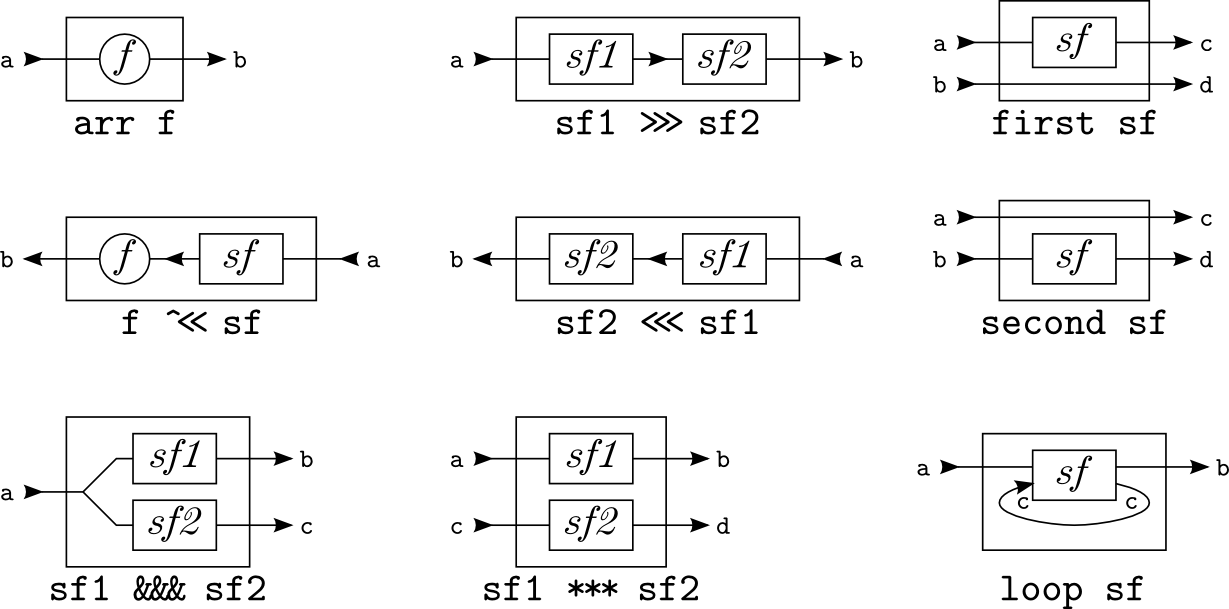
\includegraphics[width=0.9\textwidth]{graphs/yampasf.png}
\label{fig:arrowcombinators}
\end{center}
\end{figure}

  AFRP está basado en \textit{Arrows} \cite{hughes1998:arrows}
una generalización del concepto de \textit{Monads}. En particular
\texttt{SF} es una instancia de la clase \textit{Arrow}.

  Un programa es una \texttt{SF} global, compuesta por un conjunto
de otras \textit{Signal functions}, y un intérprete corre ésta instancia
global.

  En la Figura \ref{fig:arrowcombinators} se puede ver un conjunto
extenso de combinadores, sin embargo se
puede definir un conjunto minimal utilizando sólo
los combinadores \texttt{arr},
$\gg$ y \texttt{first}, aunque no es el único.

  \paragraph{Yampa}
  El framework \textit{Yampa} \cite{yampa} embebido en Haskell, 
define los operadores de la Figura \ref{fig:arrowcombinators}
para combinar señales y aplicar funciones sobre ellas.



%TODO(Marcos): Ejemplos de los operadores y su uso?



\subsection{Elm: Programación funcional reactiva concurrente}


Por último existe un lenguaje llamado Elm \cite{evanczaplicki2012:Elm},
creado para poder escribir aplicaciones web reactivas
de una forma funcional declarativa.
  En Elm, las entradas se asumen conocidas y son dadas,
por ejemplo un click o el movimiento del mouse,
o una tecla presionada.

  Todos los valores son señales, el combinador $lift$
toma una señal y una función, y define otra señal resultado
de la aplicación de la función sobre cada valor de la señal.

  Para combinar más de una señal, se usa el combinador $lift_2$ o
$lift_n$ con $n \in N$.
  En los casos que se desea tener memoria, por ejemplo llevar una
cuenta de ocurrencias de una señal, o mantener un estado explícito,
se utiliza el combinador $foldp$.

  El combinador $foldp$ opera sobre una señal como el
operador $fold$ sobre una lista.
  Dado un valor inicial y una función, aplica la función sobre
cada valor, utilizando el último valor conocido como primer argumento.

  La Figura \ref{fig:elmexample} muestra un programa Elm de ejemplo.
  El mismo toma una señal \texttt{Mouse.position}, y dada la función
  \texttt{asText} que convierte un par de valores en texto, utiliza
  \texttt{lift} para aplicar la función a las coordenadas de un Mouse.
 
\begin{figure}[h]
  \begin{center}
  \caption{Ejemplo de programa Elm. (Imagen tomada de \cite{evanczaplicki2012:Elm})}
  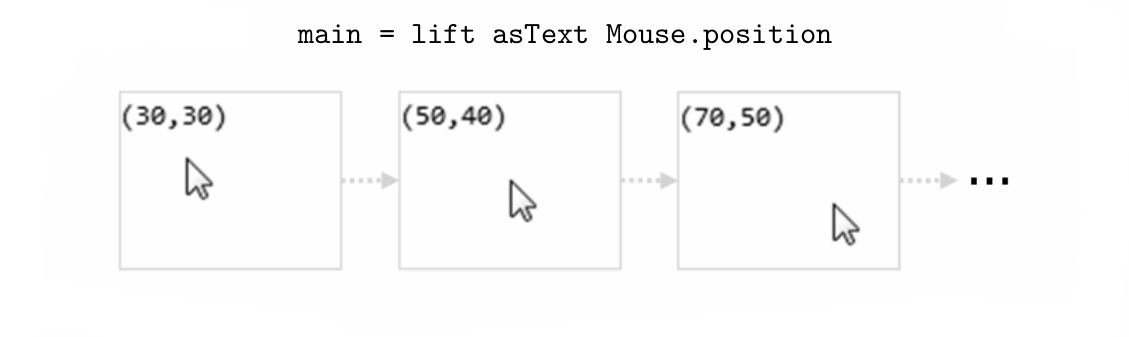
\includegraphics[width=0.9\textwidth]{graphs/elmexample.png}
  \label{fig:elmexample}
  \end{center}
\end{figure}

   
\subsection{Simplificación del paradigma}

\section{Simplificación del paradigma}

  Al intentar implementar en un computador programas utilizando éste paradigma, nos encontramos
con varias limitaciones.
  Una de ellas es que no es posible tener valores que se modifiquen de forma contínua, la capacidad
de cómputo es finita, y no es posible ejecutar tareas al mismo tiempo, incluso en un entorno con
paralelismo, el mismo está acotado a la cantidad de procesadores con los que se cuente.\\

  Aunque el paradigma distinga Eventos de Comportamientos, se puede hacer una simplificación y
asumir que todos los valores son Eventos. Los comportamientos en realidad serán una secuencia de
cambios de valor, los eventos que dependan de un comportamiento serán notificados sólo en el momento
que éste cambie.\\
  Valores como el tiempo (reloj) y otros sensores como ser un sensor de distancia, entregarán valores
periódicamente. Sería imposible que un programa reaccione a un valor contínuo, sin embargo, es muy fácil
asumir que lo que nos importa del tiempo en realidad es dada una variación de tiempo cómo se debe
comportar nuestro programa.\\
  A su vez un sensor de distancia no nos puede entregar infinitos valores, y generalmente sólo importa
poder recibir un valor nuevo en un período relativamente corto de tiempo.

  Otra limitación en nuestro caso, al tratarse de robots con bajas capacidades de cómputo, es que
la implementación del lenguaje no siempre tendrá más de un procesador disponible.\\
  Para simular éste paralelismo se asumirá que el tiempo que se necesita para hacer cálculos es de
una magnitud mucho menor al tiempo que lleva recibir un dato de una entrada, o enviar un dato a una salida.
  Se implementará una máquina capaz de correr dichos programas, la cuál esperará por valores en las entradas,
y en base a los mismos, actualizará todos los eventos que dependan de ellas, y a su vez actualizará luego
las salidas que dependan de éstos.\\
  Cada actualización se hará secuencialmente hasta terminar, y en caso de contar con más de un procesador, se
asignarán en paralelo las actualizaciones utilizando varios hilos de ejecución.\\




\subsection{Ventajas} 

  La motivación para utilizar el paradigma presentado, es que un programa reactivo escrito de
forma iterativa, es susceptible a contener errores de concurrencia al modificar valores en diferentes
rutinas. A su vez, es difícil estructurar un programa iterativo para que reaccione rápidamente a
los cambios.

  Un patrón utilizado comunmente para estructurar un programa reactivo es el patrón \texttt{Observer}.
En dicho patrón, un \texttt{Sujeto} puede ser observado por un \texttt{Observador}, éste último se
subscribe al \texttt{Sujeto}, el cuál notifica a todos sus \texttt{Observadores} cuando su valor cambia.
  
  La desventaja de hacer un programa reactivo siguiendo ese esquema, es que es difícil ver en que
momento ocurren las actualizaciones de los \texttt{Observadores}.
  Si hay muchos \texttt{Observadores} suscritos a cambios de muchos \texttt{Sujetos},
se vuelve complejo mantener el código al tener tantas interacciones implícitas.
  
  En la programación funcional reactiva, todos los valores dependientes del tiempo son observables,
la complejidad crece muy rápido y por eso deben ser elementos de primera clase.

  Al usar un lenguaje funcional, las interacciones son especificadas declarativamente, y se puede
entender como un valor es formado a partir de otros.

  Además se cumple que una función invocada con las mismas entradas en diferentes
instantes de tiempo, siempre retorna el mismo valor, lo que ayuda a razonar sobre un programa.

  Para ver que es lo que está sucediendo en un programa se pueden obtener los valores de
  todas las entradas en un instante de tiempo, como si fuera una fotografía 
  y evaluar las señales para encontrar errores o corroborar si el mismo es correcto.

  De ésta manera si un programa tiene un error, se puede tomar una secuencia de instantes,
como si fuera una grabación y entender donde está el problema claramente,
sin necesidad de seguir varios hilos de ejecución ni razonar sobre la concurrencia.


%%\subsection{Ejemplo}
%%
\begin{figure}[h!]
\begin{center}
    \caption{Ejemplo completo}
\begin{Verbatim}[frame=single]
INPUT_DISTANCE = 1
OUTPUT_ENGINE = 1

MIN_DIST = 30
MAX_SPEED = 100
STOP = 0

distanceToSpeed n = if (n < MIN_DIST) then STOP else MAX_SPEED

do {
  distance <- read INPUT_DISTANCE,
  speed <- lift distanceToSpeed distance,
  output OUTPUT_ENGINE speed
}
\end{Verbatim}
   \label{fig:example1}
\end{center}
\end{figure}

